%%%%%%%%%%%%%%%%%%%%%%%%%%%%%%%%%%%%%%%%%%%%%%%%%%%%%%%%%%%%%%%%%%%%%%%%%%%%%%
% CS110: Introduction to Computing
% Copyright 2015 Pejman Ghorbanzade <mail@ghorbanzade.com>
% Creative Commons Attribution-ShareAlike 4.0 International License
% https://github.com/ghorbanzade/UMB-CS110-2015S/blob/master/LICENSE
%%%%%%%%%%%%%%%%%%%%%%%%%%%%%%%%%%%%%%%%%%%%%%%%%%%%%%%%%%%%%%%%%%%%%%%%%%%%%%

\def \topDirectory {.}
\def \texDirectory {\topDirectory/src/main/tex}

\documentclass[12pt,letterpaper,twoside]{article}
\usepackage{\texDirectory/template/style/directives}
\usepackage{\texDirectory/template/style/assignment}
%%%%%%%%%%%%%%%%%%%%%%%%%%%%%%%%%%%%%%%%%%%%%%%%%%%%%%%%%%%%%%%%%%%%%%%%%%%%%%
% CS110: Introduction to Computing
% Copyright 2015 Pejman Ghorbanzade <mail@ghorbanzade.com>
% Creative Commons Attribution-ShareAlike 4.0 International License
% https://github.com/ghorbanzade/UMB-CS110-2015S/blob/master/LICENSE
%%%%%%%%%%%%%%%%%%%%%%%%%%%%%%%%%%%%%%%%%%%%%%%%%%%%%%%%%%%%%%%%%%%%%%%%%%%%%%

\course{id}{CS110}
\course{name}{Introduction to Computing}
\course{venue}{Tue/Thu, 5:30 PM - 6:45 PM}
\course{semester}{Spring 2015}
\course{department}{Department of Computer Science}
\course{university}{University of Massachusetts Boston}

\instructor{name}{Pejman Ghorbanzade}
\instructor{title}{}
\instructor{position}{Student Instructor}
\instructor{email}{pejman@cs.umb.edu}
\instructor{phone}{617-287-6419}
\instructor{office}{S-3-124B}
\instructor{office-hours}{Tue/Thu 19:00-20:30}
\instructor{address}{University of Massachusetts Boston, 100 Morrissey Blvd., Boston, MA}


\begin{document}

\doc{title}{Assignment 2}
\doc{date-pub}{Feb 17, 2015 at 5:30 PM}
\doc{date-due}{Mar 03, 2015 at 5:30 PM}
\doc{points}{8}

\prepare{header}
\section*{Question 1}

Write a program \texttt{ShapeDiamond.java} that asks for an integer number \texttt{n} and using \texttt{*} characters, prints a diamond in \texttt{2n-1} rows, such that there is one \texttt{*} character in first row, three \texttt{*} characters in second row and $2n-1$ characters in $n$th row.
Figure \ref{fig1} shows a sample diamond created when user has entered 4 as input integer.
\begin{verbbox}
   *
  ***
 *****
*******
 *****
  ***
   *
\end{verbbox}
\begin{figure}[H]\centering
\theverbbox
\caption{Sample diamond generated in 7 rows} \label{fig1}
\end{figure}

\section*{Question 2}

Remember the Dalton Brothers? Neglecting their original heights, write a program \texttt{Daltons2.java} that asks for heights of Joe, William, Jack and Averell, as well as the order in which they have to be sorted in terms of height. The order is either \texttt{ASC} for shortest to tallest or \texttt{DESC} for tallest to shortest. The program should give names of the brothers in order of their heights as specified.
\newpage

\section*{Question 3}

\begin{wrapfigure}{r}{0.5\textwidth}
\centering
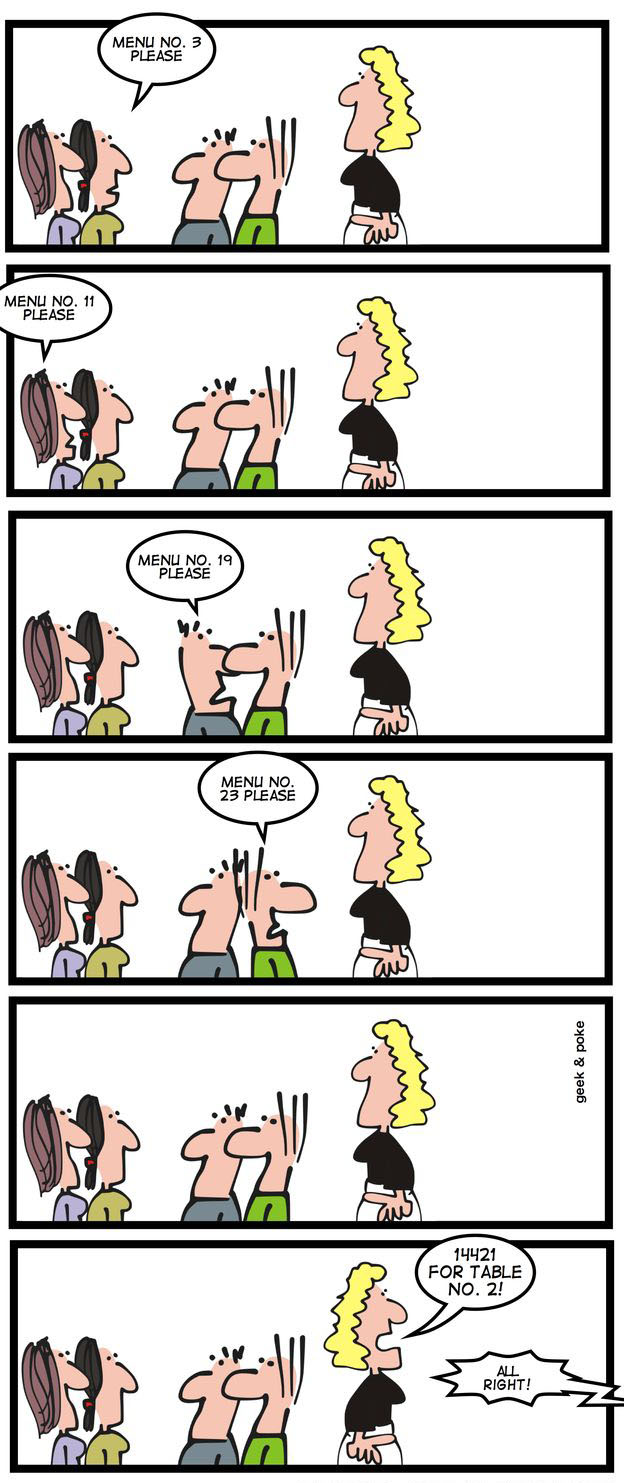
\includegraphics[width=0.5\textwidth]{\texDirectory/template/images/primeMenu.jpg}
\end{wrapfigure}

Minnie and Mannie are students of mathematics. Their area of interest is prime numbers. They also work part time in a restaurant. To fight the extreme boredom of their routine tasks at work, they have invented a little somewhat challenging game between themselves.

Minnie, the waitress, has numbered each item in the menu with a unique \textbf{random} prime number. When Minnie takes orders of a table, she will multiply the menu numbers of all orders placed by that table and gives the final multiplication to Mannie, the chef.

Thanks to his brilliant mind, Mannie will in less than two seconds decompose the given number to its prime factors and prepares the menu numbers corresponding to those factors.

Unfortunately, Mannie is absent this week and you have to replace him. As it is likely that you cannot decompose a number as fast as Mannie, you are requested to write a program \texttt{PrimeMenu.java} that asks for an integer number and prints all prime factors that number is divisible by. Obviously, your program should also indicate how many times the number is divisible by each prime number.

\end{document}
